% ---------------------------------------------------------------------------
% Automatically generated by make_tex.py from baseline.csv — do not edit.
% Build:  pdflatex baseline.tex
% ---------------------------------------------------------------------------
\documentclass[11pt,a4paper]{article}
\usepackage[margin=2cm,landscape]{geometry}
\usepackage[T1]{fontenc}
\usepackage{booktabs}
\usepackage{amssymb}
\usepackage[dvipsnames]{xcolor}
\usepackage{pgfplots}
\pgfplotsset{compat=1.18}
\usepgfplotslibrary{groupplots}

\begin{document}
\pagestyle{empty}

\section*{CVRP — published baselines}

Test sets from Ma, Cao \& Chee, \emph{Learning to Search Feasible and
Infeasible Regions of Routing Problems with Flexible Neural k-Opt},
NeurIPS 2023 (arXiv:2310.18264), tables 1 and 12.
Gaps are relative to HGS, which serves as the reference.
Times are the published ones, for the complete set.

\bigskip

\begin{center}
\small
\begin{tabular}{lll rrr rrr rrr}
\toprule
& & & \multicolumn{3}{c}{$N=20$} & \multicolumn{3}{c}{$N=50$} & \multicolumn{3}{c}{$N=100$} \\
\cmidrule(lr){4-6} \cmidrule(lr){7-9} \cmidrule(lr){10-12}
Method & Type & Post & Obj. & Gap (\%) & Time & Obj. & Gap (\%) & Time & Obj. & Gap (\%) & Time \\
\midrule
  HGS [21] & H & -- & 6.130 & -- & 10.7h & 10.366 & -- & 1.2d & 15.563 & -- & 2.5d \\
  LKH-3 [20] & H & -- & 6.135 & 0.08 & 17.9h & 10.375 & 0.09 & 2.8d & 15.647 & 0.54 & 5.7d \\
  \addlinespace
  NeuOpt-GIRE (D2A=1, T=1k) & L2S/RL & -- & 6.132 & 0.03 & 4m & 10.430 & 0.61 & 12m & 15.865 & 1.94 & 28m \\
  NeuOpt-GIRE (D2A=1, T=5k) & L2S/RL & -- & 6.130 & 0.00 & 20m & 10.382 & 0.16 & 59m & 15.698 & 0.87 & 2.3h \\
  NeuOpt-GIRE (D2A=1, T=10k) & L2S/RL & -- & 6.130 & 0.00 & 41m & 10.375 & 0.08 & 2h & 15.656 & 0.60 & 4.6h \\
  NeuOpt-GIRE (D2A=5, T=6k) & L2S/RL & -- & 6.130 & 0.00 & 2.1h & 10.369 & 0.03 & 5.9h & 15.610 & 0.30 & 13.8h \\
  NeuOpt-GIRE (D2A=5, T=20k) & L2S/RL & -- & 6.130 & 0.00 & 6.8h & 10.367 & 0.01 & 19.7h & 15.586 & 0.15 & 1.9d \\
  NeuOpt-GIRE (D2A=5, T=40k) & L2S/RL & -- & 6.130 & 0.00 & 13.7h & 10.367 & 0.01 & 1.6d & 15.579 & 0.10 & 3.8d \\
  \addlinespace
  Sym-NCO [13] (A=8, T=200) & L2C/RL & -- & -- & -- & -- & -- & -- & -- & 15.702 & 0.89 & 7.2h \\
  POMO [4] (A=8, T=200) & L2C/RL & -- & 6.136 & 0.09 & 11m & 10.397 & 0.30 & 1.4h & 15.672 & 0.70 & 7.2h \\
  POMO+EAS [5] (A=8, T=200) & L2C/RL & AS & 6.132 & 0.04 & 38m & 10.379 & 0.13 & 3.1h & 15.610 & 0.30 & 16h \\
  POMO+EAS+SGBS [34] (short) & L2C/RL & AS+BS & -- & -- & -- & -- & -- & -- & 15.587 & 0.15 & 1d \\
  POMO+EAS+SGBS [34] (long) & L2C/RL & AS+BS & -- & -- & -- & -- & -- & -- & 15.579 & 0.10 & 4.1d \\
\bottomrule
\end{tabular}
\end{center}

\bigskip

\begin{center}
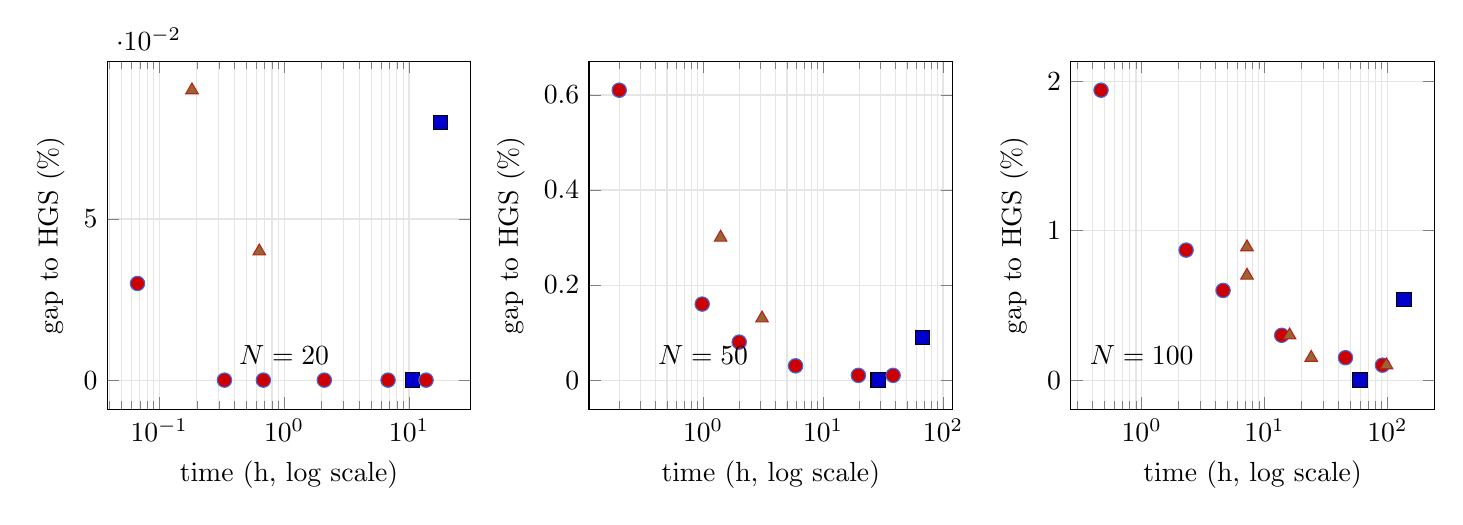
\begin{tikzpicture}
  \begin{groupplot}[
      group style={group size=3 by 1, horizontal sep=1.5cm},
      width=6.2cm, height=6cm,
      xmode=log, xlabel={time (h, log scale)},
      ylabel={gap to HGS (\%)},
      grid=both, grid style={gray!20},
      every axis title/.style={above,yshift=2pt},
      /tikz/mark size=2.6pt,
    ]
    \nextgroupplot[title={$N=20$}]
      \addplot+[only marks,mark=square*,  draw=black,      fill=black!15] coordinates {(10.7,0) (17.9,0.08)};
      \addplot+[only marks,mark=*,        draw=RoyalBlue,  fill=RoyalBlue!30] coordinates {(0.067,0.03) (0.333,0) (0.683,0) (2.1,0) (6.8,0) (13.7,0)};
      \addplot+[only marks,mark=triangle*,draw=BrickRed,   fill=BrickRed!30] coordinates {(0.183,0.09) (0.633,0.04)};
    \nextgroupplot[title={$N=50$}]
      \addplot+[only marks,mark=square*,  draw=black,      fill=black!15] coordinates {(28.8,0) (67.2,0.09)};
      \addplot+[only marks,mark=*,        draw=RoyalBlue,  fill=RoyalBlue!30] coordinates {(0.2,0.61) (0.983,0.16) (2,0.08) (5.9,0.03) (19.7,0.01) (38.4,0.01)};
      \addplot+[only marks,mark=triangle*,draw=BrickRed,   fill=BrickRed!30] coordinates {(1.4,0.3) (3.1,0.13)};
    \nextgroupplot[title={$N=100$}]
      \addplot+[only marks,mark=square*,  draw=black,      fill=black!15] coordinates {(60,0) (136.8,0.54)};
      \addplot+[only marks,mark=*,        draw=RoyalBlue,  fill=RoyalBlue!30] coordinates {(0.467,1.94) (2.3,0.87) (4.6,0.6) (13.8,0.3) (45.6,0.15) (91.2,0.1)};
      \addplot+[only marks,mark=triangle*,draw=BrickRed,   fill=BrickRed!30] coordinates {(7.2,0.7) (7.2,0.89) (16,0.3) (24,0.15) (98.4,0.1)};
  \end{groupplot}
\end{tikzpicture}

\medskip
\footnotesize
\textcolor{black}{$\blacksquare$}~Classical (H) \quad
\textcolor{RoyalBlue}{$\bullet$}~Learn-to-search \quad
\textcolor{BrickRed}{$\blacktriangle$}~Learn-to-construct
\end{center}

\vfill
\footnotesize
13 methods. Bottom-left = better (fast and close to HGS).
HGS sits at zero gap by construction; its cost is its computation time.

\end{document}
